\documentclass[conference]{IEEEtran}
\IEEEoverridecommandlockouts
% The preceding line is only needed to identify funding in the first footnote. If that is unneeded, please comment it out.
\usepackage{cite}
\usepackage{amsmath,amssymb,amsfonts}
\usepackage{algorithmic}
\usepackage{graphicx}
\usepackage{textcomp}
\usepackage{xcolor}
\def\BibTeX{{\rm B\kern-.05em{\sc i\kern-.025em b}\kern-.08em
    T\kern-.1667em\lower.7ex\hbox{E}\kern-.125emX}}
\begin{document}

\title{Project \#15: Twitter hate speech detection 2\\
}

\author{\IEEEauthorblockN{Janne Eskola\\janne.eskola@student.oulu.fi}

\and
\IEEEauthorblockN{Teemu Ikävalko\\Teemu.Ikavalko@student.oulu.fi}

\and
\IEEEauthorblockN{Toni Kuosmanen\\toni.kuosmanen@student.oulu.fi}

\and
\IEEEauthorblockN{Tapio Kursula\\t.kursula@gmail.com}

}

\maketitle

\begin{abstract}
We experimented with several possible methods for detecting hate speech on the Twitter 
platform. Approaches utilizing sentiment analysis did not perform as well as expected but 
we got better results using topic and named entity analysis. We also tested a possible metric 
for measuring the radicalization of a Twitter user but more effort needs to be made to 
validate the proposed metric.
\end{abstract}

\begin{IEEEkeywords}
natural language processing, sentiment analysis, hate speech
\end{IEEEkeywords}
\section{Introduction}
The Cambridge dictionary defines hate speech as:
\vspace{12pt}
\emph{``public speech that expresses hate or encourages violence towards a person or group based on something
such as race, religion, sex, or sexual orientation''} \cite{Cambridge:hate_speech}
\vspace{12pt}

In practice, defining clear boundaries between hate speech and normal expression can be
hard. Legal definitions of hate speech vary by country with some countries setting much
stricter definitions of hate speech. \cite{Wikipedia:hate_speech_laws}

It could be argued that today, the largest platforms for public speech are provided by 
the social media companies, such as Facebook or Twitter. Both these companies forbid 
hate speech on their platforms \cite{Twitter:hate_speech,Facebook:hate_speech} but the sheer volume 
of posted content makes it hard to enforce these rules. The services rely on users reporting
hateful content when it is found on the platform. Facebook has also utilized machine learning
algorithms in detecting hate speech but the results have not been optimal. \cite{Time:facebook_hate_speech_languages}

Hate speech can be spread by individuals or extremist groups seeking to advance their 
agendas. Hate speech is usually directed at minorities with the aim of demonizing and 
dehumanizing the targeted group. The effects of hate speech can be severe. For example, the 
UN fact finding mission sent to Myanmar, after the government crackdown on the Rohingya 
minority, found that hate speech spread on Facebook contributed significantly to sparking 
tensions in the region\cite{Reuters:myanmar_rohingya}.

The goal of our project is to find efficient methods for identifying hate speech in online forums.
Specifically, we will target the Twitter platform. We will use the Twitter search API to retrieve and then 
manually label a hate speech data set. By examining this data set, we aim to find a potential set of features 
that could be used to identify hate speech content.  We will also profile individual posters who actively spread 
hate speech on Twitter.

\section{Problem description}
Our investigation consists of two parts. In the first part we will collect a tweet data set by searching 
for tweets with specific hashtags. This data set will be manually labeled as either hate or 
non-hate speech. We will then characterize the tweets in both categories using following features:

\begin{itemize}
    \item Sentiment analysis
    \item LIWC features
    \item Emoticon usage
    \item Named entity usage
\end{itemize}

For the second part we will identify three active twitter accounts that frequently post 
hate speech content. We will analyze the posting history of these users and calculate a 
proposed radicalization score for each user. 

\section{Data sets}
\subsection{Data set 1: Labeled hate speech}
The first data set was collected using five specific hashtags, given to us in the assignment,
that were likely targets for hate speech. The hashtags were the following: 
\begin{itemize}
    \item \#bombing
    \item \#extremist
    \item \#islamophobia
    \item \#radicalist
    \item \#terrorist    
\end{itemize}

The tweets were collected using the Twitter premium search API with 30 day history. Retweets 
and tweets not written in English were excluded from the search. Our goal was to retrieve at least 
200 tweets per hashtag but we set the upper limit at 500. The tweets were saved as JSON files. 
After the tweets were retrieved through the API, they were labeled manually. The labels were appended  
to the original JSON schema so that all information could be preserved. 
A summary of the labeled data set is shown in table 
\ref{tab:data_set_1_summary}.

\begin{table}[!ht]
    % Add some padding to the table cells:
    \def\arraystretch{1.2}%
    \begin{center}
      \caption{Data set 1 summary}
      \label{tab:data_set_1_summary}
      \begin{tabular}{l c c c}
        \hline\hline
        &\multicolumn{3}{c}{\textbf{Number of tweets}} \\
        \textbf{\textit{Hashtag}}& \textbf{\textit{Non-hate speech}}& \textbf{\textit{Hate speech}} & \textbf{\textit{Total}}  \\
        \cline{2-4} 
        \hline
        \#bombing & 195 & 2 & 197\\
        \#extremist & 368 & 6 & 374\\
        \#islamophobia & 158 & 12 & 170\\
        \#radicalist & 13 & 0 & 13\\
        \#terrorist & 334 & 117 & 451\\
        \hline
        \textbf{TOTAL} & \textbf{1068} & \textbf{137} & \textbf{1205}\\
        \hline
      \end{tabular}  
    \end{center}
  \end{table}

As can be seen from the table, some topics yielded very few tweets we would label as hate speech 
while some of the hashtags, especially \#radicalist, were barely used at all. We found the largest
proportion of hate speech with the terrorist hashtag (Fig \ref{fig:data_set_1_summary}). The final 
data set contained a total of 1205 tweets out of which 137 were labeled as hate speech. 

\begin{figure}[htbp]
\centering
\centerline{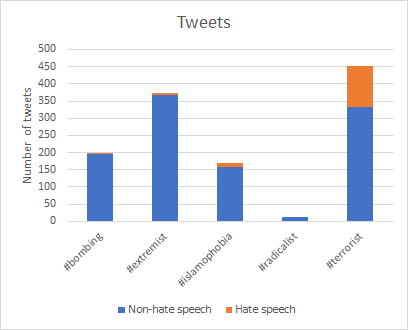
\includegraphics[width=2.5in]{data_set_1_summary.png}}
\caption{Hate/non-hate tweets per each hashtag.}
\label{fig:data_set_1_summary}
\end{figure}

\subsection{Data set 2: Active hate speakers}
For the second data set, we looked for active twitter users who frequently posted hate speech content. 
The search was limited to English speaking users only. In the end, we chose three users who fit our 
criteria: 
\begin{itemize}
    \item User 1: An UK citizen and a blogger frequently posting hate speech targeted at Muslims.
    \item User 2: Active Finnish user frequently posting racist content.
    \item User 3: A former leader of an American white supremacist group.
\end{itemize}
After selecting the users, we used Twitters full archive API to retrieve thousand tweets from each user for the
radicalization analysis. 
\section{Methods}
\subsection{Sentiment analysis}
For sentiment analysis we were tasked with plotting the percentage of polarity for both the 
annotated hate speech posts and non-hate speech posts and comparing results from two different 
sentiment analyzers. We chose Textblob \cite{python:textblob} and VADER \cite{hutto2014vader,python:vader} Python toolkits for performing the analysis. 
Both of these tools give sentiment score values between -1 and 1. We analyzed all tweets using
both libraries and divided them in to three categories based on the sentiment scores: 

\begin{itemize}
  \item negative:   [-1.000, -0.333[
  \item neutral:    [-0.333,  0.333]
  \item positive    ]0.333, 1.000] 
\end{itemize}

URLs and user names were removed from the tweets before analysis. The resulting sentiment 
percentages are summarized in table \ref{tab:sentiment_anaylysis_summary}. Polarity percentages 
are also plotted in figures \ref{fig:textblob_sentiments} and \ref{fig:vader_sentiments}

\begin{table}[!ht]
  % Add some padding to the table cells:
  \def\arraystretch{1.2}%
  \begin{center}
    \caption{Sentiment analysis}
    \label{tab:sentiment_anaylysis_summary}
    \begin{tabular}{l  c c | c c} 
      \hline\hline
      % \multicolumn{2}{c}{\textbf{non-hate speech}} 
      &\multicolumn{2}{c}{\textbf{Texblob}}&\multicolumn{2}{c}{\textbf{VADER}}\\
      \cline{2-5}
      \textbf{Sentiment}&\textbf{Hate}&\textbf{Non-hate}&\textbf{Hate}&\textbf{Non-hate}\\
      \hline
      Positive&77\%&78\%&31\%&44\%\\
      Neutral&12\%&13\%&31\%&24\%\\
      Negative&11\%&9\%&37\%&32\%\\
      \hline
      \hline      
    \end{tabular}  
  \end{center}
\end{table}

\begin{figure}[htbp]
  \centering
  \centerline{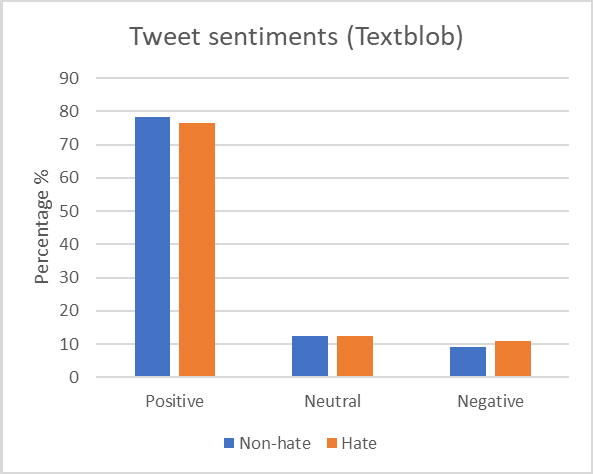
\includegraphics[width=2.5in]{Textblob.png}}
  \caption{Tweet sentiment percentages in hate and non-hate tweets (Texblob)}
  \label{fig:textblob_sentiments}
  \end{figure}

  \begin{figure}[htbp]
    \centering
    \centerline{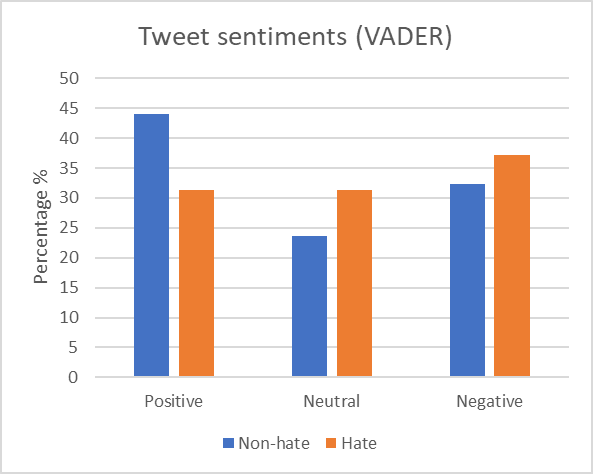
\includegraphics[width=2.5in]{Vader.png}}
    \caption{Tweet sentiment percentages in hate and non-hate tweets (Vader)}
    \label{fig:vader_sentiments}
    \end{figure}

% Analysis was performed so that every tweet that we had was cleaned so that only the text part of tweets remained. The 
% text  were then split to hate speech and non-hate speech and were then imported to both sentiment analyzers and result were compared.

\subsection{LIWC features}
To identify common themes and topics in the labeled tweet data set, we 
used Empath, which is an open-source alternative to proprietary LIWC software  \cite{fast2016empath}. 
The library offers tools that can extract themes and topics from a given text.
The library comes with a default set of categories but new categories can be added by the users. 
Our analysis uses the default categories.

Before the analysis, we removed the URLs and user names from the tweets. After cleaning, we analyzed each tweet text individually using Empath and counted the frequency of extracted topics in both the hate and non-hate categories. 
These raw counts were then normalized by dividing them with the number of tweets in the category. The normalized 
scores for the twenty most common topics are presented in tables \ref{tab:liwc_features_non_hate} 
and \ref{tab:liwc_features_hate}. Bar plots of the most common topics can also be found in the appendix.

\begin{table}[!ht]
    % Add some padding to the table cells:
    \def\arraystretch{1.2}%
    \begin{center}
      \caption{Top 20 most common topics in non-hate tweets}
      \label{tab:liwc_features_non_hate}
      \begin{tabular}{l c | c c}
        \hline\hline
        % \multicolumn{2}{c}{\textbf{non-hate speech}} 
        \multicolumn{4}{c}{\textbf{Non-hate speech}}\\
        \hline
        \textbf{Topic}&\textbf{Score}&\textbf{Topic}&\textbf{Score}\\
        \hline
        negative\_emotion&0.1713&terrorism&0.0927\\
        war&0.1573&weapon&0.089\\
        fight&0.1311&positive\_emotion&0.0871\\
        speaking&0.1301&violence&0.0758\\
        crime&0.1264&power&0.074\\
        communication&0.1124&business&0.0712\\
        government&0.1105&giving&0.0693\\
        aggression&0.1105&hate&0.0684\\
        kill&0.1067&law&0.0665\\
        politics&0.0946&leader&0.0655\\
        \hline\hline
      \end{tabular}  
    \end{center}
  \end{table}

  \begin{table}[!ht]
    % Add some padding to the table cells:
    \def\arraystretch{1.2}%
    \begin{center}
      \caption{Top 20 most common topics in hate speech tweets}
      \label{tab:liwc_features_hate}
      \begin{tabular}{l c | c c}
        \hline\hline
        % \multicolumn{2}{c}{\textbf{non-hate speech}} 
        \multicolumn{4}{c}{\textbf{Hate speech}}\\
        \hline
        \textbf{Topic}&\textbf{Score}&\textbf{Topic}&\textbf{Score}\\
        \hline
        negative\_emotion&0.2847&crime&0.1168\\
        hate&0.2701&appearance&0.1168\\
        children&0.219&speaking&0.1095\\
        family&0.2117&fight&0.1095\\
        love&0.2044&government&0.1022\\
        youth&0.1898&giving&0.0949\\
        emotional&0.1752&disgust&0.0949\\
        affection&0.1752&communication&0.0949\\
        kill&0.1679&terrorism&0.0876\\
        war&0.1168&leader&0.0876\\
        \hline\hline
      \end{tabular}  
    \end{center}
  \end{table}
\subsection{Emoticon usage}
We investigated the usage of emoticons in hate and non-hate tweets by examining the types 
of emoticons used and their frequency.  Using Emojis Python library \cite{python:emojis}, we 
listed all the distinct emoticons in every tweet. The hate speech tweets contained a total of 22 tweets which contained emoticons
while the  non-hate tweets contained 154. The percentage of tweets containing emojis was 
roughly the same in the two categories, 16 \% and 14 \% in hate and non-hate categories respectively.

The most frequent emoticons are listed in tables \ref{tab:emoticons_non_hate} and \ref{tab:emoticons_hate}. 
Bar plots of the most common emoticons can also be found in the appendix.


\begin{table}[!ht]
    % Add some padding to the table cells:
    \def\arraystretch{1.2}%
    \begin{center}
      \caption{Top 20 most common emoticons in non-hate speech tweets}
      \label{tab:emoticons_non_hate}
      \begin{tabular}{l c | c c}
        \hline\hline
        % \multicolumn{2}{c}{\textbf{non-hate speech}} 
        \multicolumn{4}{c}{\textbf{Non-hate speech}}\\
        \hline
        \textbf{Emoticon}&\textbf{Frequency [\%]}&\textbf{Emoticon}&\textbf{Frequency [\%]}\\
        \hline
        :end: & 5.43\% & :pout: & 0.47\%\\
        :bell: & 5.43\% & :muscle: & 0.47\%\\
        :point\_right: & 2.81\% & :heavy\_minus\_sign: & 0.37\%\\
        :joy: & 1.03\% & :calling: & 0.37\%\\
        :point\_down: & 0.66\% & :warning: & 0.28\%\\
        :wink: & 0.56\% & \emph{:sotwe:*} & 0.28\%\\
        :fire: & 0.56\% & :smirk: & 0.28\%\\
        :us: & 0.47\% & :wave: & 0.19\%\\
        :uk: & 0.47\% & :thumbsup: & 0.19\%\\
        :rofl: & 0.47\% & :smile: & 0.19\%\\                           
        \hline
        \multicolumn{4}{l}{\emph{*:stuck\_out\_tongue\_winking\_eye:}}\\
        \hline\hline
      \end{tabular}  
    \end{center}
  \end{table}

\begin{table}[!ht]
    % Add some padding to the table cells:
    \def\arraystretch{1.2}%
    \begin{center}
      \caption{Top 20 most common emoticons in hate speech tweets}
      \label{tab:emoticons_hate}
      \begin{tabular}{l c | c c}
        \hline\hline
        % \multicolumn{2}{c}{\textbf{non-hate speech}} 
        \multicolumn{4}{c}{\textbf{Hate speech}}\\
        \hline
        \textbf{Emoticon}&\textbf{Frequency [\%]}&\textbf{Emoticon}&\textbf{Frequency [\%]}\\
        \hline
        :joy: & 5.11\% & :stop\_sign: & 0.73\%\\
        :pout: & 4.38\% & :star\_of\_david: & 0.73\%\\
        :uk: & 1.46\% & :sparkler: & 0.73\%\\
        :thumbsup: & 1.46\% & :snake: & 0.73\%\\
        :smirk: & 1.46\% & :skull\_and\_crossbones: & 0.73\%\\
        :roll\_eyes: & 1.46\% & :skull: & 0.73\%\\
        :muscle: & 1.46\% & :point\_up\_2: & 0.73\%\\
        :clap: & 1.46\% & :point\_down: & 0.73\%\\
        :blush: & 1.46\% & :pensive: & 0.73\%\\
        :v: & 0.73\% & :menorah: & 0.73\%\\                        
        \hline\hline
      \end{tabular}  
    \end{center}
\end{table}

The most common emoticons used in the hate speech, :joy: and :pout:, don't really stand out 
and are frequently used in non hate context, although both seem to be more common in our 
hate speech data set. Other emoticons in the hate speech tweets were occured only once or twice.

The two most common emoticons in the non hate speech data set were :exit: and :bell:. 
It turns out both emoticons were frequently used by opponents of Jeremy Corbyn, who 
were active during the British general election that occurred in December 2019, at 
the same time we were collection our data sets.

\subsection{Named entities}
We investigated the use of named entities and their frequency in tweets containing hate 
speech and not containing hate speech. The tweets were analyzed using spaCy natural 
language processing library for python. Using the default spacy model (en\_core\_web\_sm) 
for entity recognition, we identified the 20 most used named entities in both sets of 
tweets and their frequency based on the size of the tweet set 
(Tables \ref{tab:named_entities_hate} and \ref{tab:named_entities_non_hate}).
We also plotted graphs of these entities and their frequency. The graphs can be found in 
the appenix. 

\begin{table}[!ht]
  % Add some padding to the table cells:
  \def\arraystretch{1.0}%
  \begin{center}
    \caption{Top 20 most common named entities in hate speech tweets}
    \label{tab:named_entities_hate}
    \begin{tabular}{l c | c c}
      \hline\hline
      % \multicolumn{2}{c}{\textbf{non-hate speech}} 
      \multicolumn{4}{c}{\textbf{Hate speech}}\\
      \hline
      \textbf{Entity}&\textbf{Freq. [\%]}&\textbf{Entity}&\textbf{Freq. [\%]}\\
      \hline
      UK & 0.2409 & LabourParty & 0.0511\\
      Antisemitic & 0.1168 & Communist & 0.0511\\
      Socialist & 0.0876 & Terrorist & 0.0438\\
      2019 & 0.0803 & Pakistan & 0.0438\\
      ChairmanCorbyn & 0.073 & Jews & 0.0438\\
      Nazis & 0.0584 & ComradeCorbyn & 0.0438\\
      Nazi & 0.0584 & NeverCorbyn & 0.0292\\
      JeremyCorbyn & 0.0584 & Labour & 0.0292\\
      Islamophobia & 0.0584 & ISIS & 0.0292\\
      London & 0.0511 & GeneralElection2019 & 0.0292\\                        
      \hline\hline
    \end{tabular}  
  \end{center}
\end{table}

\begin{table}[!ht]
  % Add some padding to the table cells:
  \def\arraystretch{1.2}%
  \begin{center}
    \caption{Top 20 most common named entities in non-hate speech tweets}
    \label{tab:named_entities_non_hate}
    \begin{tabular}{l c | c c}
      \hline\hline
      % \multicolumn{2}{c}{\textbf{non-hate speech}} 
      \multicolumn{4}{c}{\textbf{Hate speech}}\\
      \hline
      \textbf{Entity}&\textbf{Freq. [\%]}&\textbf{Entity}&\textbf{Freq. [\%]}\\
      \hline
      Islamophobia & 0.1152 & graffiti & 0.0403\\
      JeremyCorbyn & 0.0627 & EXTREMIST & 0.0393\\
      GeneralElection2019 & 0.0599 & HINDU & 0.0384\\
      Communist & 0.0599 & NeverCorbyn & 0.0365\\
      India & 0.059 & Pakistan & 0.029\\
      Lies & 0.0515 & Labour & 0.029\\
      RSS & 0.0468 & US & 0.0281\\
      Twat & 0.044 & Muslims & 0.0243\\
      UK & 0.0421 & berlin & 0.0234\\
      BJP & 0.0412 & Muslim & 0.0234\\                          
      \hline\hline
    \end{tabular}  
  \end{center}
\end{table}

In tweets containing hate speech frequent named entities are closely related to UK and their 
current political situation. Jeremy Corbyn, his political party and his relations with 
Pakistan were mentioned in many of the hate speech tweets.
The hate speech entity list also contains a high number of words closely associated with 
general hate speech, such as Nazi and Islamophobia. The same trend of named entities can 
be seen in the frequent entities used in tweets that did not contain hate speech. 
Many of the most frequent entities are related to United Kingdom and Jeremy Corbyn. 
Other frequent topic that can be seen in this list is the conflict between Pakistan and 
India, with entities related to these countries and their major religions, Hinduism and Islam.

\section{Radicalization of active hate speakers}
The second dataset consist of tweets from three user accounts on Twitter that are active hate-speech spreaders. Like in the first part, only English speaking users were examined.
We aggregate a thousand tweets per user and give each user a radicalization score based on the characteristics of their tweets.

We extract the following features from their tweets per user:
\begin{itemize}
  \item Average sentiment score percentile (\(AS\))
  \item Volume of negative posts (\(VN\))
  \item Severity of negative posts (\(SN\))
  \item Duration of negative posts (\(DN\))
\end{itemize}
We use the following formula to compute a radicalization score for each user
\[Radicalization\: score = (K /AS^3) \cdot (VN \cdot SN \cdot DN)\], where \(K = 1\)
%\caption{Radicalization score formula}


\(AS\): Sentiment is within the range [-1,1], where -1 is the most negative and 1 the most positive sentiment.
 This range must be normalized to [0,1] to be used as intended in the radicalization score formula.\\ %\ref{}
\(VN\): The proportion of the posts that had a negative sentiment.\\
\(SN\): The proportion of the posts that had a 'very negative' sentiment. If a posts standardized value is less than negative three, it was considered as 'very negative'.
Standardized value is acquired for each sentiment value using the following formula;
\(z = (X - \mu)/\sigma\), where \(X\) is the value in question, and \(\mu\) and \(\sigma\) are the mean and the standard deviation of the dataset that the value belongs to. Standardized values have a mean of \(0\) and a standard deviation of \(1\). This means that a standardized value of 3, for example, is three standard deviations away from the mean to the positive side.\\
\(DN\): The duration, in number of days, between the oldest and newest tweet with a negative sentiment. \\
\\
We used pythons TextBlob for calculating the sentiments of each tweet and got the results shown in table \ref{tab:radicalization_scores}.

\subsection{Results}

\begin{table}[!ht]
  \def\arraystretch{1.2}%
  \begin{center}
  \caption{Radicalization scores}

  \label{tab:radicalization_scores}
  \begin{tabular}{l | c c c}
    \hline\hline
    & User 1 & User 2 & User 3\\
    \hline
    AS & 0.525 & 0.5016 & 0.5222\\
    VN & 0.218 & 0.22 & 0.279\\
    SN & 0.014 & 0.022 & 0.012\\
    DN & 77 & 503 & 246\\
    \hline
    RS & 11 & 135 & 40\\
    \hline\hline
    
  \end{tabular}
\end{center}
\end{table}

\section{Results}

\subsection{Sentiment analysis}
The sentiment percentages we obtained using Text blob were practically identical for both 
hate and non-hate tweets. Textblob found a vast majority of the tweets, 77 \% and 78 \%
for hate and non-hate groups respectively, to be positive. Surprisingly, negative sentiment 
scores made up only about 10 \% of the Textblob sentiments. These results show that Texblob 
sentiment scores are not a good way to distinguish between hate and non hate speech.

VADER analyzer performed slightly better in discriminating between the hate and non-hate tweet sentiments.
Negative sentiments were most common in the hate speech and positive sentiments in the non-hate 
speech tweets (Fig \ref{fig:vader_sentiments}). The sentiments were more evenly distributed so that all categories were within 20\% of 
each other’s values. Still, the difference between the hate and non-hate sentiments is not 
as great as we would have predicted.

\subsection{Empath topics}
Considering the hashtags that were used to collect the tweets, 
it is not surprising that Empath found negative and violent topics present 
in both hate and non-hate categories. Still, there is a marked difference in 
the scores between the two categories. The topics in the non-hate speech category 
are more evenly distributed which is to be expected due to the difference in sample size.
Even taking this into account, the topic 'hate' is still much more pronounced in the hate speech 
data set.  Surprisingly, themes like 'children', 'family', 'love', and 'youth' are also some of the 
most common topics in the hate speech category. The difference between the two categories suggest 
that Empath topics might be useful for identifying hate speech content.

\subsection{Emoticon usage}
The most common emoticons found in the hate speech tweets are widely used and cannot be considered hateful 
without further context. Based on our data, emoticons with more specialized meanings are rarely used and 
seem poor candidates for indicators. 
Many of the hate tweets containing the emoticon :joy: were malicious and mocking. 
Detecting the misalignment between the nominal meaning of an emoticon and the actual tone of the message could 
potentially be an efficient indicator of hateful content.

\subsection{Named entities}
The most frequently used named entities in tweets studied did not differ very much between normal tweets 
and hate tweets. Named entities found in the tweets used were mainly of two types. First type are named 
entities related to current events, mainly to Brexit that is currently ongoing in United Kingdom and 
Jeremy Corbyn. Some of this type of entities were in tweets that were related to the current situation 
between Pakistan and India.

The other type was named entities that are closely related to hate speech but not necessarily to major current events. 
Examples of such entities include Nazis, Islamophobia and Terrorist.
This analysis shows that named entities are an effective way to find topics and events that generate 
hate speech content. However, differentiating between hate speech and not hate speech through this 
method is less effective since the data sets that this analysis produced are very similar. 

The results also clearly show how strongly current events can affect the type and 
frequency of named entities. The December elections in United Kingdom left a clear mark in our 
data set. If the data was gathered now, we predict several of the named entities would not be 
present. The entities that attract the most hate speech are not stable but instead might shift rapidly.

\subsection{Radicalization scores}
All of the users average sentiment percentiles were close to neutral - in fact,
all of them were slightly or somewhat positive. 
Majority of the tweets were given a neutral sentiment, which gives the users overall
a rather low radicalization score from the maximum, given the high impact that \(AS\)
has to the formula. For example, if a theoretical users variables were as follows: \(AS\) = 0.2,
\(VN\) = 0.5,\(SN\) = 0.25\(DN\) = 300, their radicalization score would be 4687.5, three orders
of magnitude higher than the scores these users got. This neutrality 
is probably partly due to the sentiment analyzers sole focus on adjectives. The sentiment analyzer
was unable to analyze more complex patterns in the tweets.
TextBlobs default sentiment analyzer uses the same implementation as the "patterns" library does,
and it has a certain drawback: it only takes adjectives into account. This lead to most of the 
tweets sentiment scores to be zero. 

We attempted to use another sentiment
analyzator, one provided by vadersentiment,
which was specifically designed to be used on social media, such as facebook or twitter. 
The analyzator, however, proved to be problematic. 
The variances of sentiments were too big when computing the \(SN\) to be in range of the sentiment, 
which is on the range [-1, 1]. The specification of the \(SN\) is the proportion of the values which 
have a standardized value smaller than -3, i.e, proportion of the values which are more than 3 standard 
deviations away from the mean to the negative side. The variances of the sentiments were so large, that 
a value so far from the mean would be out of range of the sentiment value for all of the users. This resulted 
in \(SN\) being zero, which in turn resulted for the radicalization score being zero for all of the users. 
Although the vadersentiment gave better results in the sense that it had less tweets with a neutral sentiment 
value, due to this property of the \(SN\), it's usage had to be discontinued. \\

\section{Conclusions}
We experimented with several different methods in order to find features for identifying hate speech.
The approaches employing sentiment analysis did not work as well as we predicted in distinguishing between 
normal speech and hate speech. Other methods of sentiment analysis might prove more effective.

The Empath topics showed a clear distinction between the hate and non-hate data sets. Feature vector
constructed from the topics most common to hate speech could be employed for training a model to recognize 
hate speech. Named entities could also be used though training the model might be harder since 
trending entities are so time dependent. Emoticon usage, if evaluated purely as the types of 
emoticons used, did not seem particularly effective in distinguishing hate speech. Combining 
emoticon analysis with other methods might provide better results.

It is hard to gauge how well the calculated radicalization scores reflects the actual radicalization 
of the subjects. Further more our analysis might have suffered from the poor performance of the 
Texblob sentiment analysis. More effort should be spent in the future in order to validate the metric.
Alternative tools for sentiment analysis should also be considered.

\section*{Source Code} \addcontentsline{toc}{section}{Source}
Full source code of our project, including the data sets, can be found at:
\\\\
https://github.com/tokuosma/NLP2019
\\\\
Interactive calculation of the results can be performed in the Jupyter notebook 
also included in the repository.

\bibliographystyle{IEEEtran}
\bibliography{IEEEabrv,project_15}
\vspace{12pt}

\appendix

\begin{itemize}
    \item Figure 4 : Empath categories in the hate speech and non-hate speech tweets 
    \item Figure 5 : Emoticon usage in the hate speech and non-hate speech tweets 
    \item Figure 6 : Named entities in hate speech tweets
    \item Figure 7 : Named entities in non-hate speech tweets
\end{itemize}

\begin{figure*}[!t] 
\centering 
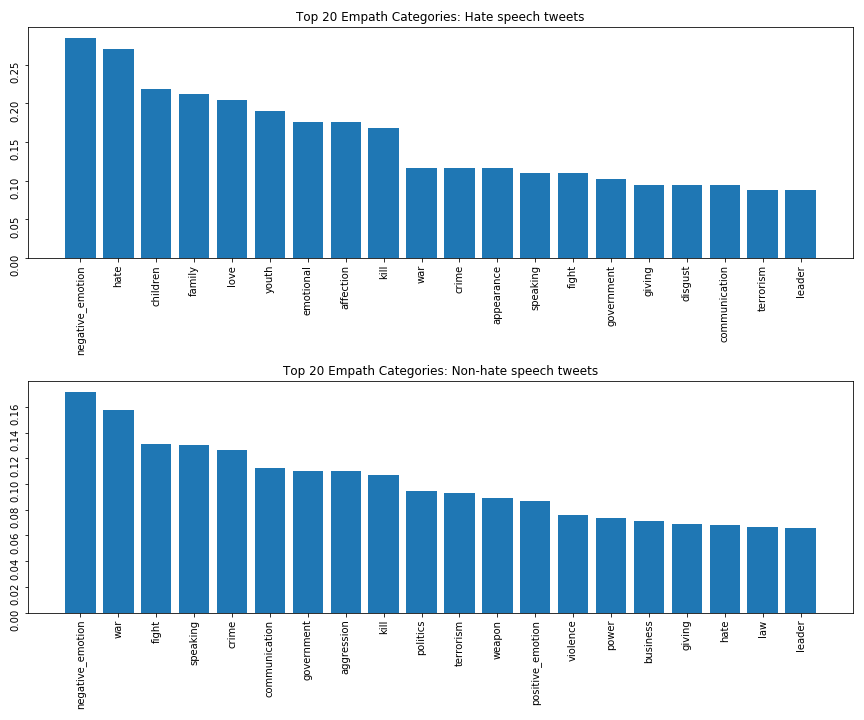
\includegraphics[width=5.0in]{liwc_topics} \label{fig:liwc_topics} \hfil 
\caption{Empath categories in the hate speech and non-hate speech tweets.}     
\end{figure*} 

\begin{figure*}[!t] 
    \centering 
    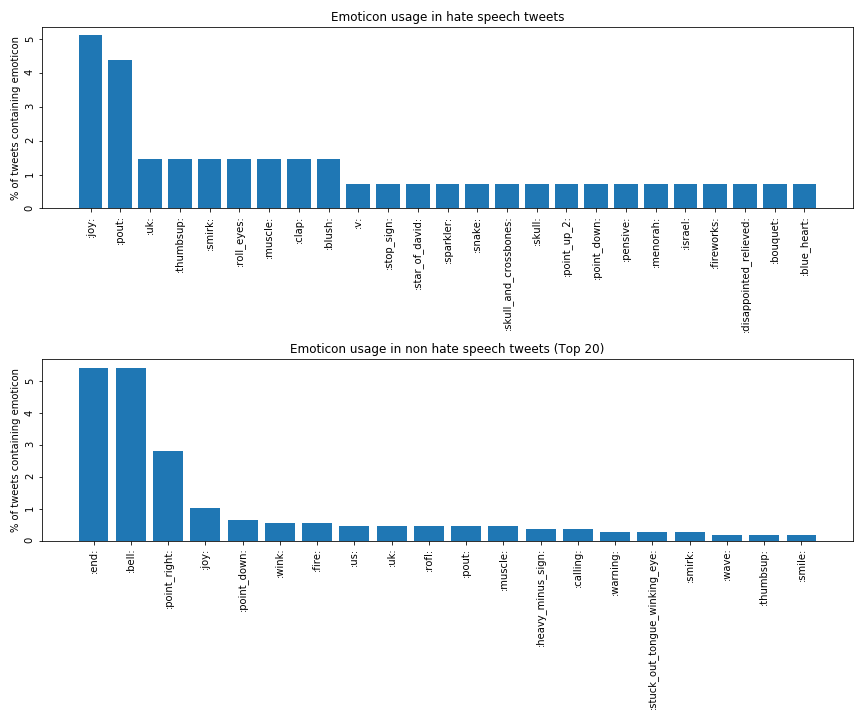
\includegraphics[width=5.0in]{emoticons} \label{fig:emoticon_usage} \hfil 
    \caption{Emoticon usage in the hate speech and non-hate speech tweets.}     
\end{figure*} 

\begin{figure*}[!t] 
  \centering 
  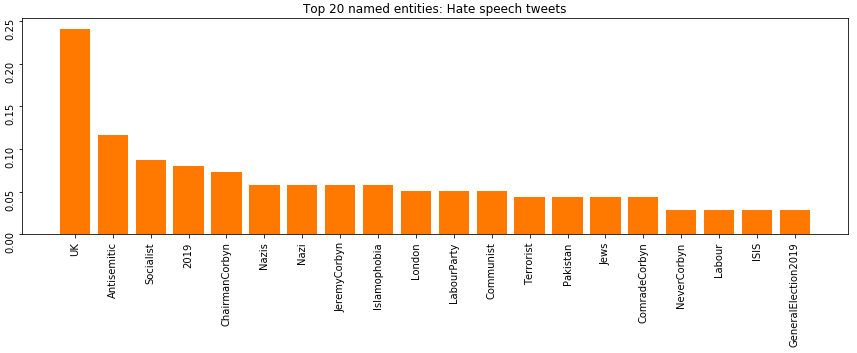
\includegraphics[width=5.0in]{entities_hate} \label{fig:entities_hate} \hfil 
  \caption{Named entities in hate speech tweets}     
\end{figure*} 


\begin{figure*}[!t] 
  \centering 
  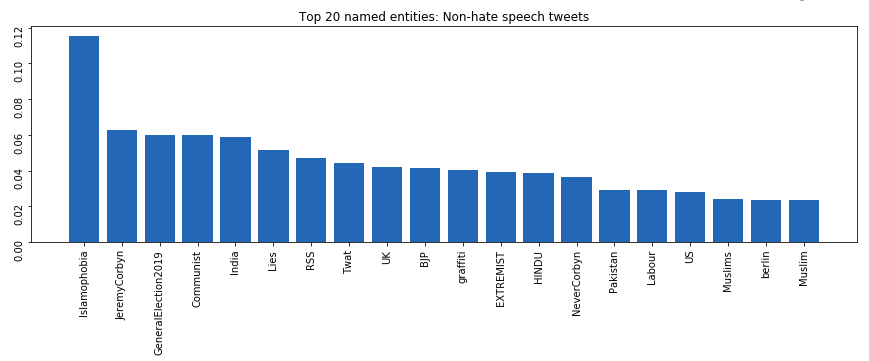
\includegraphics[width=5.0in]{entities_no_hate} \label{fig:entities_non_hate} \hfil 
  \caption{Named entities in non-hate speech tweets}     
\end{figure*} 

\end{document}
    
    
